\chapter{Introduction}\label{cha:intro}

Data processing is required by every modern business in some form. Existing solutions like SQL fit the requirements of the majority of use cases, as the volume of data they process can be contained within a single system. However, as the volumes of data begin to increase, in particular over around 100GB of raw data, single system solutions like SQL begin to struggle as not all of the data can be loaded into memory at once. 

Figure \ref{fig:single-system-solution} shows the network model when using a single system to perform data processing on a SQL server. A number of clients are all connected to a single server, and the server can become overloaded if a large number of clients are making intensive queries, or if some of the queries operate on a large amount of data. This results in significantly reduced query performance, or even outright failure, because the system must spend a large amount of time moving data in and out of memory to complete the computation. It is possible to make extremely powerful servers, but ultimately these solutions are constrained to a single machine, meaning there is an upper limit to the compute performance based on the current technology available.

\begin{figure}[h]
	\centering
	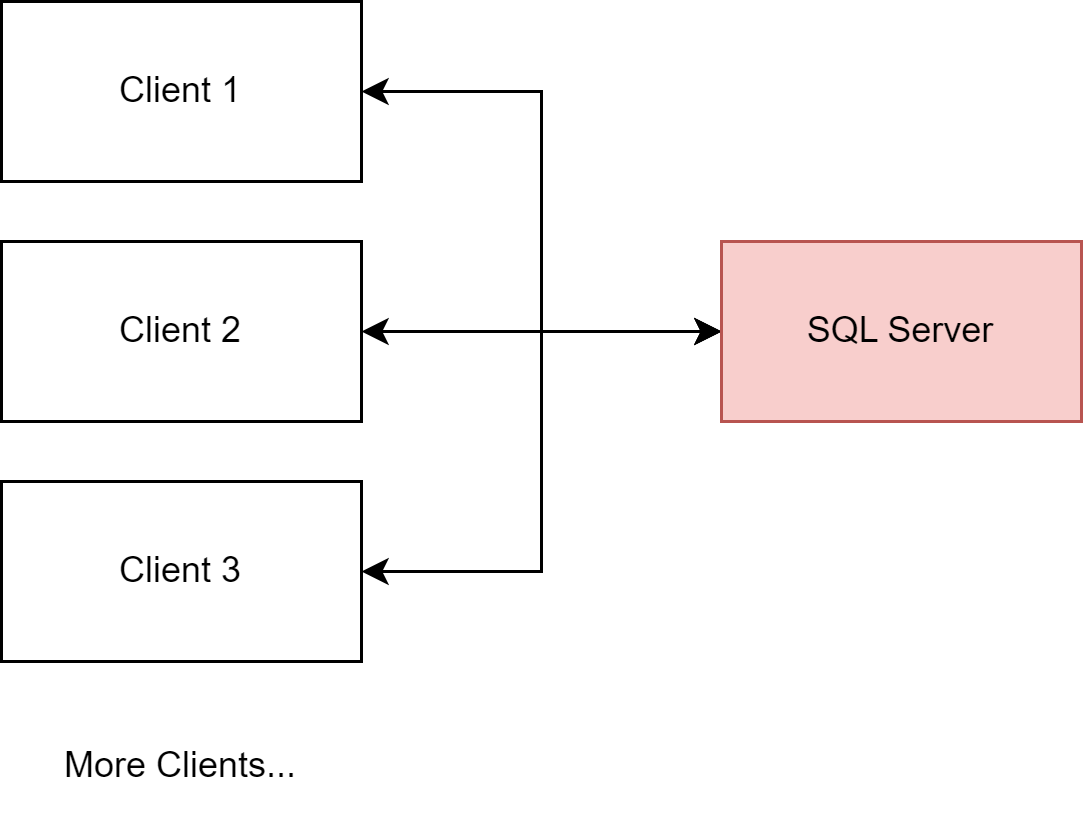
\includegraphics[width=0.4\textwidth]{chapters/diagrams/design/single-system-solution}
	\caption{Single System Solution}
	\label{fig:single-system-solution}
\end{figure}

This type of processing is generally used in \textit{extract-transform-load} (ETL) workflows, which describe the type of workflow where data must be imported in bulk from an external source, processed in some way, then exported elsewhere for further analysis. Often, the processing to be performed acts on small groups of rows in the original dataset at once, usually a unit item like a loan, customer, or product. As a result, even if the overall dataset is extremely large, the processing can be easily parallelised, as only a small number of rows are needed at any one time to produce the required output.

Distributed systems therefore present an excellent opportunity for solving this problem. If a system can be designed to automatically split a dataset up and perform the processing over a number of nodes in a cluster, this system could potentially be able to process data of any size; larger datasets can be accommodated by simply increasing the number of nodes. Similarly, performance can be scaled by increasing the number of nodes.

% Why is this area important, why am I investigating it
% More general big data references here - difficulties faced due to larger than memory data sets
% References to ETL if possible, and how this is an increasingly important workflow.

\section{Prior Work}
Distributed Data Processing has existed conceptually since as early as the 1970s. A paper by Philip Enslow Jr{\frenchspacing.} from this period sets out characteristics across three 'dimensions' of decentralisation: hardware (the number of machines involved in the computation), control (the management of the cluster), and database (decentralisation of storage) \cite{enslow1978distributed}. Enslow argued that these dimensions defined a distributed system, but acknowledged that the technology of the period was not equipped to fulfil these goals. Further research into distributed data processing can be split into two categories \cite{yaqoob2016big}:
\begin{itemize}
	\item \textbf{Batch processing:} data is gathered, processed and output all at the same time. This includes solutions like MapReduce and Spark \cite{dean2008mapreduce, zaharia2016spark}. Batch processing works best for data that can be considered 'complete' at some stage.
	\item \textbf{Stream processing:} data is processed and output as it arrives. This includes solutions like Apache Flink, Storm, and Spark Streaming \cite{carbone2015flink, toshniwal2014storm, armbrust2018sparkstreaming}. Stream processing works best for data that is being constantly generated, and needs to be analysed in real-time.
\end{itemize}

MapReduce, a framework introduced by Google in the mid 2000s, could be considered the breakthrough framework for performing massively scalable, parallelised data processing \cite{dean2008mapreduce}. It later became one of the core modules for the Apache Hadoop suite of tools. MapReduce provides a simple API, where developers could describe a job as a \textit{map} and a \textit{reduce} step, and the framework would handle the specifics of managing the distributed system. While MapReduce was Google's offering, other large technology companies released similar solutions, including Microsoft with DryadLINQ in 2009 \cite{fetterly2009dryadlinq}.

MapReduce was not without flaws, and papers were published in the years following its release which completed performance benchmarks, analysing its strengths and weaknesses \cite{lee2012parallel}. Crucially, MapReduce appears to struggle with iterative algorithms which are executed over a number of steps, as it relies on reading and writing to a persistent storage format after each step. A number of popular extensions to MapReduce were introduced to improve iterative algorithm performance, like Twister and HaLoop, in 2010 \cite{ekanayake2010twister, bu2010haloop}.

MapReduce was challenging to use for developers familiar with more traditional data processing tools like SQL due to its imperative programming style, resulting in the introduction of many tools to improve its usability. Hive is one example, featuring a SQL-like language called HiveQL that allowed users to write declarative programs, compiling into MapReduce jobs \cite{thusoo2010hive}. Pig Latin is similar, with a mixed declarative and imperative  style \cite{olston2008pig}. 
%Further tools in the wider areas of the field were introduced around 2010, including another project by Google named Pregel, specialised for performing distributed data processing on large-scale graphs \cite{malewicz2010pregel}. % probably doesn't add anything

% Spark - initial creation, talk specifically about RDDs
In 2010, the first Spark paper was released \cite{zaharia2010spark}. Spark aims to improve upon MapReduce's weaknesses, by storing data in memory and providing fault tolerance by tracking data 'lineage'. For any set of data, Spark knows how it was constructed from another persistent data source, and can use that to reconstruct lost data in failure scenarios. This in-memory storage, known as a resilient distributed dataset (RDD) allows Spark to improve on MapReduce's performance for iterative jobs, whilst also allowing it to quickly perform ad-hoc queries for interactive usage \cite{zaharia2012rdd}. This approach was successful at resolving MapReduce's weakness for iterative algorithms, as keeping the data in-memory removes the read-write overhead. 

% Spark - extensions - SQL, Streaming
Spark quickly grew in popularity, with a number of extensions being added to improve its usability, including a SQL-style engine featuring a query optimiser, and an engine supporting stream processing \cite{armbrust2015sparksql, armbrust2018sparkstreaming}. A second paper released in 2016 stated that Spark was used by thousands of organisations, with the largest deployment running an 8,000 node cluster containing 100PB of data \cite{zaharia2016spark}. Spark is designed to be agnostic of any particular storage mechanism, instead utilising existing Apache Hadoop connectors to retrieve data from various sources \cite{rddprogrammingguide}. This provides the advantage that Spark can interface with a large number of data sources, but it is not specialised for any of them, presenting an opportunity for a new solution to improve on importing data through close integration with the persistent storage.

% Stream processing tools - not entirely what I'm looking at, but still within the field - Kafka, Storm
More recent research indicates that the field is moving away from batch processing towards stream processing. A 2015 paper by Google argues that increasing data volumes, the fact that datasets can no longer ever be considered 'complete', along with demands for improved data analytics means that streaming 'dataflow' models are the way forward  \cite{akidau2015dataflow}. Google publicly stated in their 2014 'Google I/O' Keynote that they were phasing out MapReduce in their internal systems \cite{googleio2014}. 
% "the system" -> what system? I didn't get these 2 sentences. The text above says that streaming models are the way forward, but this here says that it is not required?
Streaming solutions appear to be the direction of the wider industry, but they are more suited for datasets where data is produced and must be processed at a constant rate. This project is specifically aimed at implementing a generic framework for bulk processing large, complete datasets. Therefore, while a streaming solution is not in scope for the core project, there is an opportunity for further investigation into this as an extension.

% Summarise contributions in this section (testing), summarise main challenges
\section{Project Aims}
The main objective is to design a query processing engine to perform data processing over a distributed cluster of nodes. To ensure accessibility for users of existing tools, the system should feature a SQL-like interface implemented in a widely-used language, which will allow it to be used for ETL workflows, where large data volumes often cause problems. Finally, as this will be designed as an all-in-one solution, the system should attempt to exploit the integration between the storage mechanism and cluster nodes to improve execution speed. This appears to be an area where existing distributed data processing solutions could be improved. Details of the design and implementation of the solution are described in Chapters \ref{cha:design} and \ref{cha:implementation}.

Once complete, the implementation should be assessed in a number of ways. Testing against a single-system solution like SQL Server should be conducted, along with further tests to determine the impact of varying the level of parallelisation in the cluster. Chapter \ref{cha:testing} provides full details of the tests.

\section{Challenges}
The project presents a number of key challenges that must be solved. The component which splits the dataset up will need to cope with small and large data volumes effectively, and the component which delegates parts of the full dataset to nodes in the cluster will have to handle clusters with any number of nodes correctly. The user's interface must be simple to use and understand, but expressive enough so the user can define any computation they need to. Finally, the persistent storage mechanism must be carefully selected to provide performance benefits when loading source data into the cluster.
